%FOR PDFLATEX USE ONLY
\documentclass[a4paper,12pt]{article}

\usepackage{amssymb,amsmath}

\usepackage[margin=2cm]{geometry}
\usepackage[unicode]{hyperref}
\usepackage[pdftex]{graphicx}
\usepackage{cmlgc}

\usepackage{array}

\usepackage{wrapfig}
\usepackage{array}
\usepackage{lipsum}
\usepackage{esvect}
\usepackage{hyperref}

\usepackage{subfig}
\usepackage{calc}
\usepackage{pgfplots,tikz,circuitikz}
\usepackage{pgfplotstable}
\usepackage{tkz-euclide}

\usepackage{centernot}
\usepackage{cancel}

\usepackage{mathtext}
\usepackage[T1,T2a]{fontenc}
\usepackage[utf8]{inputenc}
\usepackage[english, bulgarian, russian]{babel}
\usepackage{tikz}
\usepackage{pgfplots}
\usepackage[export]{adjustbox}
\usepackage[left=2cm,right=2cm,
    top=2cm,bottom=2cm,bindingoffset=0cm]{geometry}
\usepackage{indentfirst}
\usepackage{braket}
\usepackage{booktabs}

\begin{document}

\begin{center}
  \LARGE{Работа 2.1.6}\\[0.2cm]
  \LARGE{Эффект Джоуля–Томсона}\\[0.2cm]
  \large{Малиновский Владимир}\\[0.2cm]
  \normalsize{\texttt{galqiwi@galqiwi.ru}}
\end{center}

\textbf{Цель работы:} 1) Определение изменения температуры углекислого газа при проте-кании через малопроницаемую перегородку при разных начальных значениях давления и температуры 2) Вычисление по результатам опытов коэффициентов Ван-дер-Ваальса $a$ и $b$.

\textbf{В работе используются:} трубка с пористой перегородкой, труба Дьюара, термостат, термометры, дифференциальная термопара, микровольтметр, балластный баллон, манометр.

\section*{Описание работы}

В этой работе наблюдается эффект джоуля-томсона при прохождении углекислого газа через пористую перегородку. Эффект представляет из себя изменение температуры газа на выходе из перегородки в связи с его неидеальностью. При малых перепадах давления можно считать, что энтальпия одного моля проходящего газа сохраняется, поскольку скорости на входе и выходе отличаются не сильно:
$$\Delta M=\frac{\mu}{2} v^2,$$
при том, что $\Delta M$ -- вклад скорости частиц в энтальпию. При диаметре трубки в $3\text{мм}$ и скороcти потока порядка $10\text{мл}/\text{с}$, скорость получается порядка $\approx 1.4\,\text{м}/\text{с}$. Это меняет разность температур не сильнее, чем на:

$$\Delta T=\Delta M\,C_p=\frac{\mu}{2C_p}v^2\approx0.5\text{мК},$$

что много меньше разности температур в эксперименте ($\approx1\text{К}$).Если записать равенство энтальпий на границах перегорaодки и применить уравнение газа Ван-дер-Ваальса, можно получить связь между разницей давлений и температур:
$$\mu\text{д-т} = \frac{\Delta T}{\Delta P} = \frac{2a/(RT) - b}{C_p},$$
где $a$ и $b$ -- коэффициенты газа Ван-дер-Ваальса. В этой работе планируется получить значения $a$ и $b$ из эксперементельной зависимости $\mu\text{д-т}$ от температуры и этой формулы.

\newpage
Схема установки представлена на рис. 1:
\begin{center}
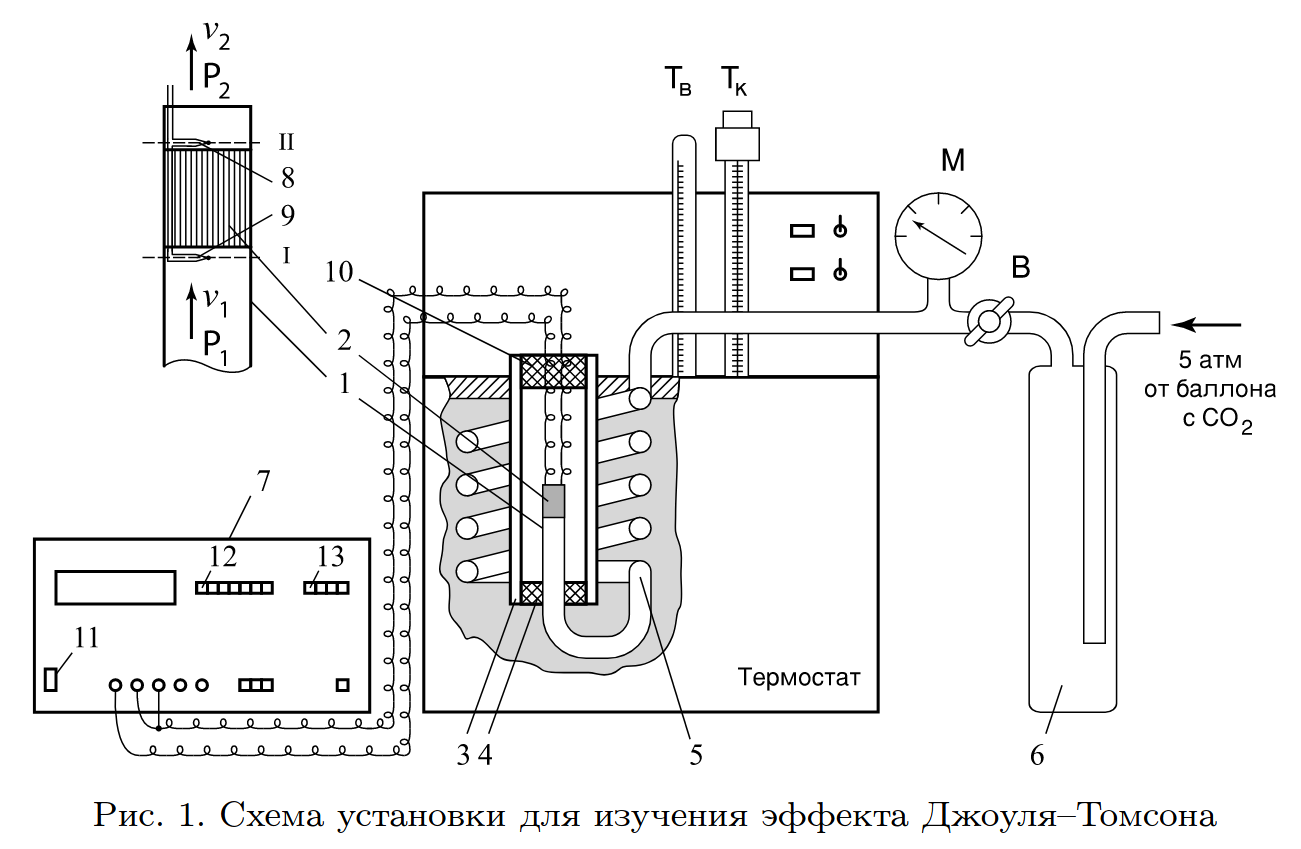
\includegraphics[width=0.95\textwidth]{equip.png}
\end{center}

\begin{enumerate}
	\item трубка с пористой перегородкой (2)
	\item пористая перегородка
	\item труба Дьюара
	\item кольцо
	\item змеевик
	\item балластный баллон
	\item вольтметр
	\item верхний спай термопары
	\item нижний спай термопары
	\item пробка из пенопласта
\end{enumerate}
\newpage
\section*{Методика и результаты}

\subsection*{1-2}
\subsection*{3}
Включим установку. Запишем начальное напряжение $V_0$ на вольтметре при $\Delta P = 0$. В дальнейшем будем учитывать это напряжение как сдвиг при измерении напряжения:
$$V = V_\text{изм} - V_0.$$
\subsection*{4-7}
\begin{enumerate}
\item Проведем измерения на температуре $T$:\\
Откроем вентиль так, чтобы избыточное давление в системе было $\approx4\,\text{бар}$. Подождем 10 минут установления равновесия в системе.
\item начнем уменьшать давление. При каждом изменении давления, подождем 5 минут установки равновесия.
\item по МНК определим значение $\mu = dT/dP = dT/dV \cdot dV/dP$.
\end{enumerate}

\subsection*{8-10}
повторим прошлый пункт для температур от комнатной до $60\,^\circ C$

\begin{center}\begin{tabular}{ccc}\begin{tabular}{|c|c|c|} \hline$p,\,\text{бар}$ & $V,\,\text{$\mu$В}$ & $T,\,\text{К}$ \\ \hline$4.00$&$137.0$&$20.640$\\ \hline $3.50$&$119.0$&$20.640$\\ \hline $3.00$&$98.0$&$20.830$\\ \hline $2.50$&$75.0$&$20.790$\\ \hline $2.00$&$57.0$&$20.850$\\ \hline \end{tabular}&\begin{tabular}{|c|c|c|} \hline$p,\,\text{бар}$ & $V,\,\text{$\mu$В}$ & $T,\,\text{К}$ \\ \hline$4.00$&$131.0$&$29.340$\\ \hline $3.50$&$112.0$&$29.570$\\ \hline $3.00$&$92.0$&$29.710$\\ \hline $2.50$&$73.0$&$29.680$\\ \hline $2.00$&$52.0$&$29.680$\\ \hline \end{tabular}&\begin{tabular}{|c|c|c|} \hline$p,\,\text{бар}$ & $V,\,\text{$\mu$В}$ & $T,\,\text{К}$ \\ \hline$4.00$&$130.0$&$40.060$\\ \hline $3.50$&$105.0$&$40.070$\\ \hline $3.00$&$86.0$&$40.050$\\ \hline $2.50$&$69.0$&$40.040$\\ \hline $2.00$&$50.0$&$40.020$\\ \hline \end{tabular}\\ \\\begin{tabular}{|c|c|c|} \hline$p,\,\text{бар}$ & $V,\,\text{$\mu$В}$ & $T,\,\text{К}$ \\ \hline$4.00$&$115.0$&$50.000$\\ \hline $3.50$&$101.0$&$50.010$\\ \hline $3.00$&$81.0$&$50.030$\\ \hline $2.50$&$66.0$&$50.040$\\ \hline $2.00$&$53.0$&$50.030$\\ \hline \end{tabular}&\begin{tabular}{|c|c|c|} \hline$p,\,\text{бар}$ & $V,\,\text{$\mu$В}$ & $T,\,\text{К}$ \\ \hline$4.00$&$105.0$&$60.000$\\ \hline $3.50$&$91.0$&$60.000$\\ \hline $3.00$&$78.0$&$60.000$\\ \hline $2.50$&$58.0$&$60.020$\\ \hline $2.00$&$48.0$&$60.010$\\ \hline \end{tabular}&\\\end{tabular}\end{center}
$$\Delta p = 0.05\,\text{бар}, \Delta V = 0.5\,\mu V, \Delta T = 0.005\,\text{К}.$$
Учет приборной погрешности:
$$\delta(dV/dT) = \sqrt{\delta(dV/dT)_\text{мнк}^2 + (\frac{\sigma_V}{<V>} + \frac{\sigma_T}{<T>})^2}.$$
Величины $dV/dT$ брались как среднее арифметичесе этой величины на участках, разделенных температурой, кратной десяти. Погрешность считалась половина соответствующего модуля разности.\\
\begin{center}
\begin{tabular}{|c|c|c|c|c|}
\hline
$T, \text{К}$&$dV/dP, \mu\text{В}/\text{бар}$&$dV/dT, \mu\text{В}/\text{К}$&$\mu = dT/dP, \text{К}/\text{бар}$&$1000\text{К}/T$\\
\hline
$293.90\pm0.05$&$40.80\pm0.89$&$40.25\pm0.45$&$1.01\pm0.03$&$3.4025\pm0.0005$\\ \hline
$302.75\pm0.07$&$39.40\pm0.53$&$41.15\pm0.45$&$0.96\pm0.02$&$3.3031\pm0.0007$\\ \hline
$313.20\pm0.01$&$39.20\pm1.35$&$42.05\pm0.45$&$0.93\pm0.04$&$3.1929\pm0.0001$\\ \hline
$323.17\pm0.01$&$31.80\pm1.06$&$42.90\pm0.40$&$0.74\pm0.03$&$3.0943\pm0.0001$\\ \hline
$333.16\pm0.01$&$29.40\pm1.21$&$43.70\pm0.40$&$0.67\pm0.03$&$3.0016\pm0.0001$\\ \hline
\end{tabular}
\end{center}

\subsection*{11-13}
Коэффициенты $a$ и $b$ можно получить, проанализировав линейную зависимость $\mu$ от $1/T$, что мы и сделаем:
\begin{center}
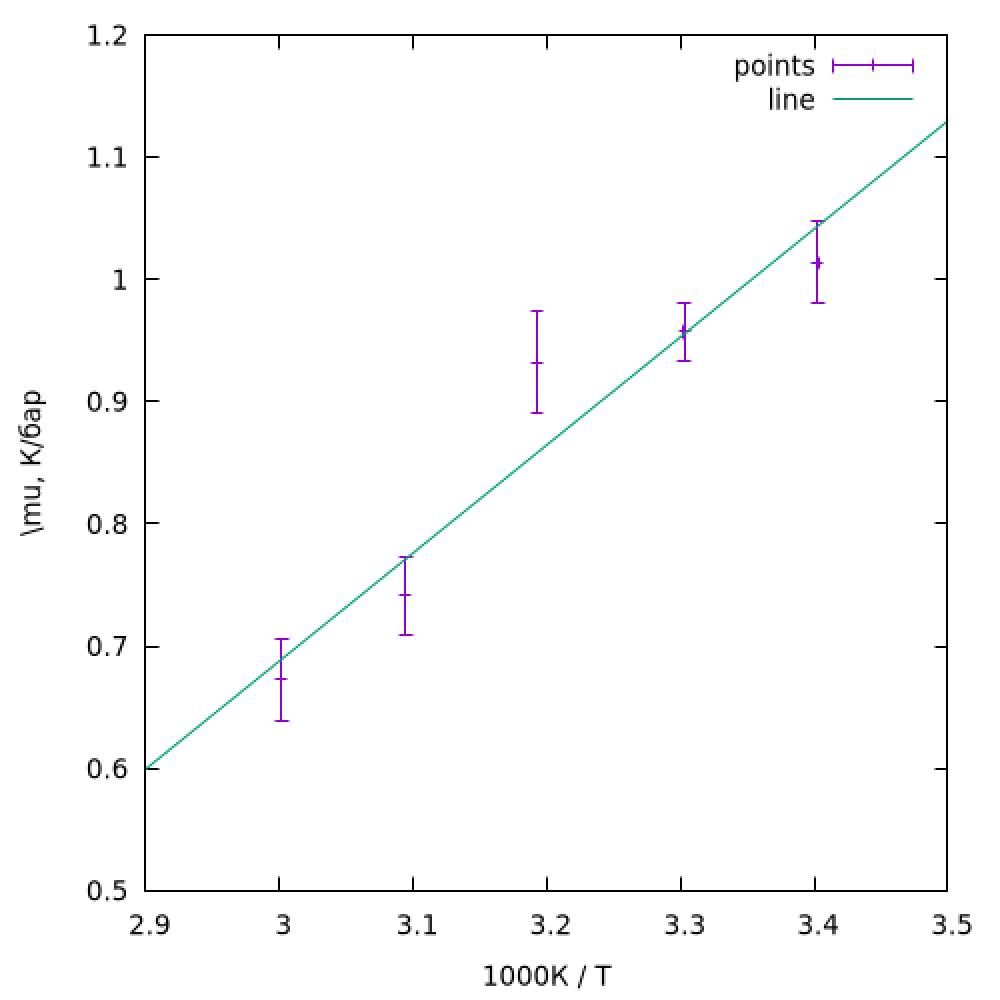
\includegraphics[width=0.95\textwidth]{plot0.png}
\end{center}
Из МНК следует, что
$$\mu = -(1.96\pm0.02)\frac{\text{К}}{\text{бар}} + (0.88\pm0.12)\frac{\text{К}}{\text{бар}}\cdot\frac{1000\text{К}}{T}.$$
Если учитывать погрешность линейного члена аналогично рассмотренной на странице раньше, а приборную погрешность постоянной добавки, как среднее арифметическое $\sigma_\mu$, то получатся коэффициенты:
$$\mu = -(1.96\pm0.07)\frac{\text{К}}{\text{бар}} + (0.88\pm0.15)\frac{\text{К}}{\text{бар}}\cdot\frac{1000\text{К}}{T}.$$
Найдем $a$, $b$:
$$a = \frac{C_pR}{2}(880\pm120)\frac{\text{К}^2}{\text{бар}}=2R^2(880\pm120)\frac{\text{К}^2}{\text{бар}} = (1.2\pm0.2) \text{Н}\text{м}^4/\text{моль}^2,$$
$$a_\text{теор} = 0.36 \text{Н}\text{м}^4/\text{моль}^2.$$
$$b = C_p(1.96\pm0.07)\frac{\text{К}}{\text{бар}}=(650\pm20)\text{см}^3/\text{моль},\,b_\text{табл} = 43\text{см}^3/\text{моль}.$$
$$T_\text{инв}=\frac{2a}{Rb}=(4.4\pm0.9)\cdot 10^2\,\text{К},\,T_\text{инв|табл}=2.0\text{кК}$$
\section*{Вывод}
Наша модель плохо описывает поведение системы, поскольку финальные коэффициенты не сошлись с табличными. Не смотря на это, они отличались от них меньше, чем в 20 раз, что не так плохо. Мы измерили изменение температуры углекислого газа при протекании через перегородку при различных давлениях и температурах и вычеслили значения коэффициентов Ван-дер-Ваальса и температуры инверсии, хоть и не точно.
\end{document}








\lipsum[1-4]
\begin{wrapfigure}{R}{5cm}
\centering
\includegraphics[width=0.20\textwidth]{rd.png}
\caption{1}
\end{wrapfigure}
\lipsum[1-6]


\begin{figure}[h]
\begin{center}$
\begin{array}{cccc}
\includegraphics[width=0.20\textwidth]{rd.png}&
\includegraphics[width=0.20\textwidth]{rd.png}&
\includegraphics[width=0.20\textwidth]{rd.png}&
\includegraphics[width=0.20\textwidth]{rd.png}\\
(1) & (2) & (3) & (4)
\end{array}$
\end{center}
\end{figure}
